\documentclass[a4paper,russian]{article}
\usepackage[utf8]{inputenc}
\usepackage[english,russian]{babel}
\usepackage[14pt]{extsizes}

%\usepackage{pscyr}
\usepackage{subfigure}
\usepackage{wrapfig}
\usepackage{cmap}
\usepackage{indentfirst}
\usepackage{autonum}
\usepackage{amsfonts}
\usepackage{amsmath}
\usepackage{amssymb}
\usepackage{amsthm}
\usepackage{upgreek}
\usepackage{graphicx}
\usepackage{listings}
\usepackage{multirow}
\usepackage{multicol}
\usepackage{dsfont}
\usepackage{graphicx}
\usepackage{caption}
\usepackage{setspace,amsmath}

\usepackage[unicode, pdftex]{hyperref}
\usepackage[left=30mm, top=20mm, right=15mm, bottom=20mm, footskip=10mm]{geometry}

\begin{document}
	\selectlanguage{russian}
\setcounter{page}{0}

\begin{center}
	\small{Министерство науки и высшего образования Российской Федерации}\\
	\small{Федеральное государственное бюджетное образовательное учреждение}\\
	\small{Высшего образования}\\
	\small{\textbf{«Северо-Осетинский государственный университет\\
			имени Коста Левановича Хетагурова»}}\\
	
	\hfill \break
	\hfill \break
	\hfill \break
	\hfill \break
	\hfill \break
	\hfill \break
	\hfill \break
	\hfill \break
	\hfill \break
	\hfill \break
	\hfill \break
	\hfill \break
	\hfill \break
	
	\normalsize{Дипломная работа}\\
	\large{\textbf{Seq2Seq - подход для реализации машинного перевода}}\\
	
	\hfill \break
	\hfill \break
	\hfill \break
	\hfill \break
	\hfill \break
	\hfill\break
\end{center}

\begin{flushright}
	\textbf{Выполнил:}\\
	Студент 4 курса направления:\\
	«Прикладная математика и информатика»\\
	\textit{Гамосов Cтанислав Станиславович \underline{\hspace{3cm}}}\\
\end{flushright}

\hfill

\begin{flushright}
	\textbf{Научный руководитель:}\\
	Кандидат физико-математических наук:\\
	\textit{Басаева Елена Казбековна \underline{\hspace{3cm}}}\\
\end{flushright}

\hfill

\begin{flushright}
	\textbf{Консультант}\\
	Старший преподаватель: \\
	\textit{Макаренко Мария Дмитриевна \underline{\hspace{3cm}}}\\
\end{flushright}

\normalsize{ \hspace{28pt}} \hfill \break
\begin{center} Владикавказ 2022 \end{center}
\thispagestyle{empty}
\clearpage
	\thispagestyle{empty}
\tableofcontents
\thispagestyle{empty}
\clearpage
\newtheorem{theorem}{Теорема}
	
	\section{Введение}
	
	\textbf{Seq2seq} - это семейство подходов машинного обучения, используемых для обработки естественного языка. Основные задачи для которого используется данные методы: нейронный перевод, субтитры к изображениям, разговорные модели и обобщение текста.
	
	Первоначальный алгоритм, который в процессе породил целое семейство методов, был разработан \textit{Google} для использования в машинном переводе. Как уже можно заметить за последнюю пару лет коммерческие системы стали удивительно хороши в  переводе - посмотрите, например, \textit{Google Translate}, \textit{Яндекс}-переводчик, переводчик \textit{DeepL}, переводчик \textit{Bing Microsoft}.
	
	Так же \textbf{Seq2seq} технология несет в себе огромный потанцевал, помимо привычного машинного перевода между естественными языками, вполне реализуем перевод между языками программирования (\textit{Facebook AI "Глубокое обучение переводу между языками программирования"}). Поэтому возможности применений такого рода подходов довольно велики. В связи с этим под машинным переводом будет подразумеваться любая задача \textbf{Seq2seq}, если точнее, то перевод между последовательностями любой природы.
	
	\clearpage
	
	\section{Рекуррентные сети}
	
	\subsection{RNN - Recиrrent Neural Network}
	Одно из важных отличий RNN от обычных нейронных сетей это понятие времени. Под ним подразумевается последовательность входных данных $x^t$, которые поступают на вход, и их выходные результаты $y^t$, которые генерируются в дискретной последовательности временных шагов, индексируемых $t$. Получаемые последовательности могут быть конечной длины или бесконечно счетными. Когда они конечны, так называемый отрезок времени примет вид $(\overline{1, T})$. 
	
	\begin{wrapfigure}{r}{0.25\textwidth}
		\centering
		\captionsetup{justification=centering}
		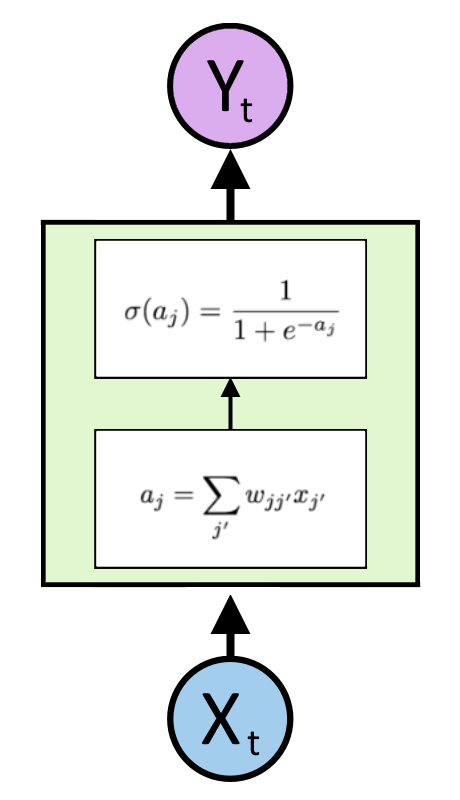
\includegraphics[height=65mm]{img/1.png}
	\end{wrapfigure}

	Таким образом, входную последовательность можно обозначить $x^t = (x^1, x^2, x^3, ... , x^T)$, а выходную последовательность как $y^t = (y^1, y^2, y^3, ... , y^T)$
	
	Рекуррентные нейронная сеть как и обычные нейронные сети представляют из себя граф состоящий из набора искусственных нейронов, обычно называемых \textbf{узлами}, и набора направленных взвешенных ребер между ними. Каждый нейрон $j$ связан \textbf{функцией активации} $\sigma_j$.
	
	\textbf{Вес} - это связь между нейронами, которая несет в себе значение, которое характеризует "важность"\ , придаваемая значению сигнала, проходящего через данное ребро или синапс. Для каждого ребра от узла $j'$ до $j$ присутствует вес $w_{jj'}$. Значение $v_j$ каждого нейрона вычисляется путем применения его функции активации к взвешенной сумме его входных данных: 
	
	$$v_j = l_j\bigg(\sum_{j'} w_{jj'} \cdot v_{j'}\bigg)$$
	
	Для удобства обозначим $a_j = \sum_{j'} (w_{jj'} \cdot v_{j'})$ и назавём \textbf{текущей активацией}. 
	\textbf{Функция активации} $\sigma(z)$ является абстракцией, представляющей скорость возбуждения нейрона. Обычно в качестве функций активации применяют:
	
	\begin{table}[h]
		\centering
		\begin{tabular}{|l|l|} 
			\hline
			Функция Хевисайда       &   
			$ H(x) = 
			\begin{cases}
				0, & x < 0 \\
				1, & x >= 0 \\
			\end{cases}$ \\ 
			\hline
			Cигмоида                &  $\sigma(x) = \frac{1}{1 + e^{-x}}$ \\ 
			\hline
			Гиперболический тангенс &  $tanh(x) = \frac{e^x - e^{-x}}{e^x + e^{-x}}$ \\ 
			\hline
			Линейный выпрямитель    &  
			$ReLU(x) =  
			\begin{cases}
				0, & x < 0 \\
				x, & x >= 0 \\
			\end{cases}$ \\
			\hline
		\end{tabular}
	\end{table}

	\clearpage
	
	\textbf{Рекуррентные Нейронные Сети (Recиrrent Neural Network - RNN)} - это класс сетей с циклами, которые хорошо подходят для обработки последовательностей. Мысли обладают неким постоянством и напрямую зависят от прошлых умозаключений. Традиционные нейронные сети на такое не способны, и это, очевидно, серьезный изъян. 
	
	Допустим перед нами стоит задача научить сеть определять эмоциональный окрас предложения, и подаём в сеть одно слово за другим. Желательно, чтобы сеть "помнила"\ уже переданные слова. Уже здесь возникает проблема обычных нейронных сетей, как же "запоминать"\ контекст? Если мы хотим, чтобы сеть переводила предложение с одного языка на другой, то тоже было бы не плохо учитывать начало, середину и конец предложение при переводе. В таких случаях именно рекуррентные нейронные сети призванны решить такие проблемы.

	В более общем плане сети RNN могут работать с последовательностями (sequence) произвольной длины, а не с входными данными фиксированного размера. Это свойство как раз таки очень важно в контексте обработки естественных языков. Также хороший пример, потому что нейронная сеть должна учитывать контекст, предоставляемый существующим предложением, чтобы завершить его.

	\begin{figure}[ht!]
		\centering
		\captionsetup{justification=centering}
		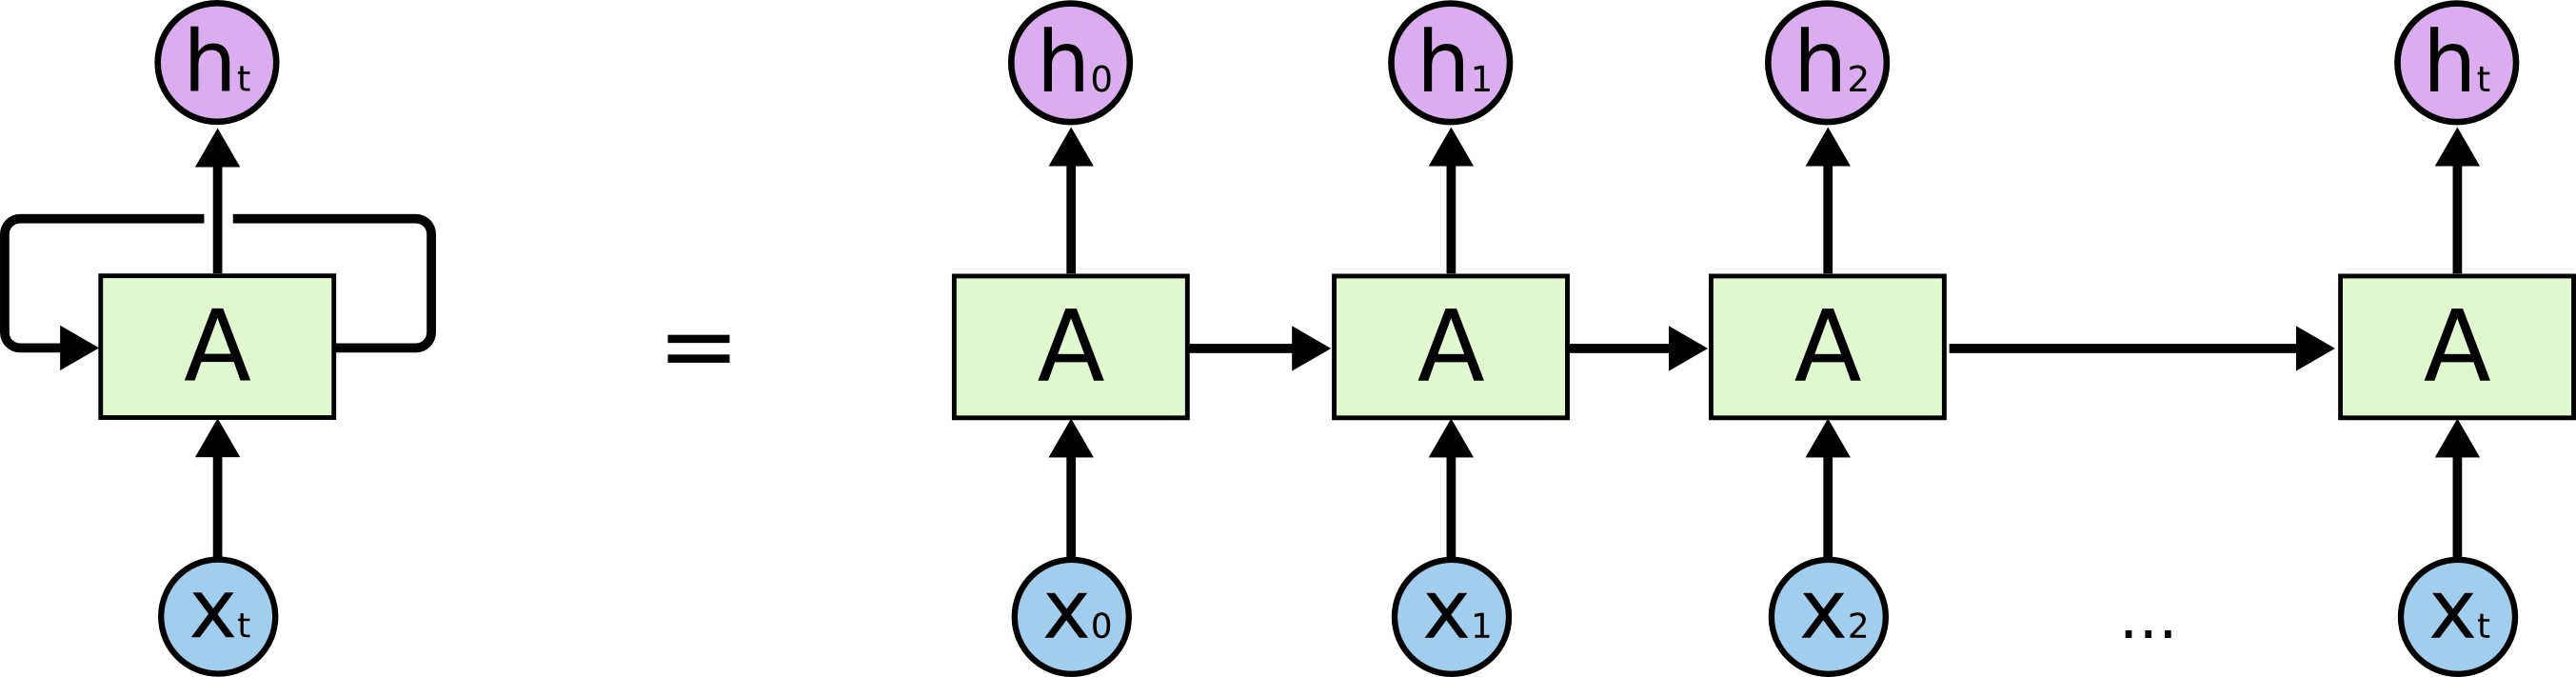
\includegraphics[height=40mm]{img/3.png}
		\caption{Развернутая рекуррентная нейронная сеть}
	\end{figure}
	
	Такая "цепная"\ сущность показывает, что рекуррентные нейронные сети по природе своей тесно связаны с последовательностями. Естественно использовать такую архитектуру для работы с этим типом данных.
	
	Кроме выходного вектора, где мы будем получать ответ, сеть должна иметь еще и некоторый вектор или векторы в, которых описывает текущее внутреннее состояние сети, т.е. в нем содержатся воспоминания о всех уже отсмотренных сетью элементах. Более формально это выглядит так.
	
	Пусть у нас есть входная последовательность $(x_{1}, x_{2}, x_{3} ..., x_{n})$, данную последовательность стоит преобразовать:
	
	$$	h^{(t)} = \sigma(w^{(hx)} \cdot x^{(t)} + w^{(hh)} \cdot h^{(t - 1)} + b_h) $$
	$$	y^{(t)} = w^{(yh)} \cdot h^{(t)} + b_y $$
	
	При этом кроме выхода $y^(t)$, мы имеем еще вектор $h^{(t)}$, описывающий текущее состояние. Таким образом сеть состоит из ячеек вида:
	
	\begin{figure}[ht!]
		\centering
		\captionsetup{justification=centering}
		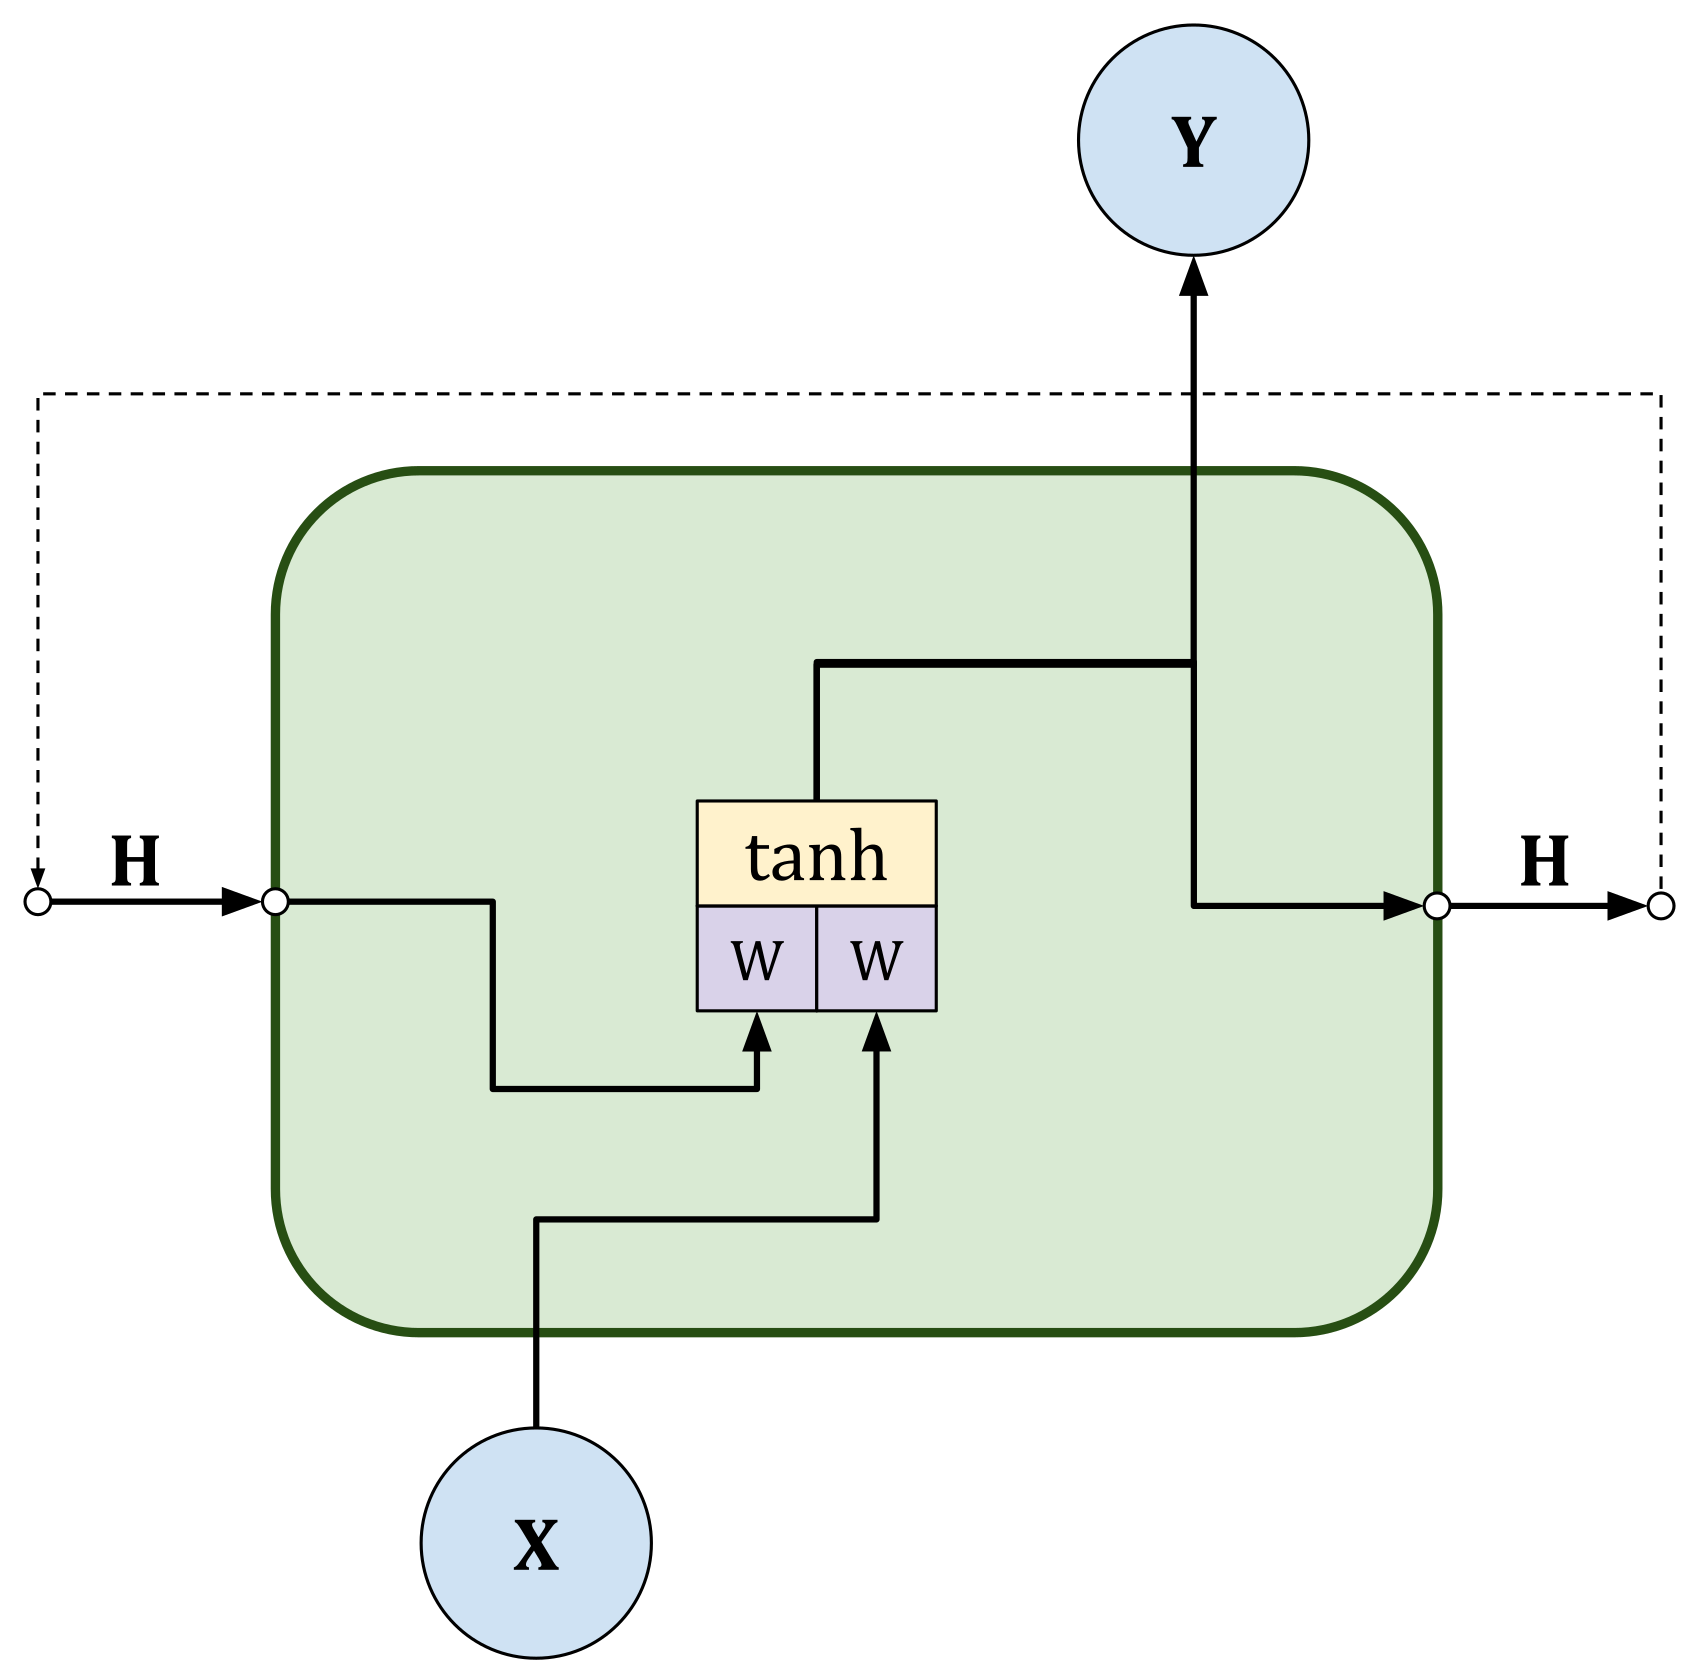
\includegraphics[height=60mm]{img/rnn_with_recurrent_link.png}
	\end{figure}
	
	Которые собираются в последовательность, передавая внутреннее состояние из ячейки в следующую за ней по времени. Отметим, что веса при этом у всех ячеек одни и теже:

	Ещё один вариант, когда сеть преобразует последовательность в последовательность, может быть вот таким:
	
	\begin{figure}[ht!]
		\centering
		\captionsetup{justification=centering}
		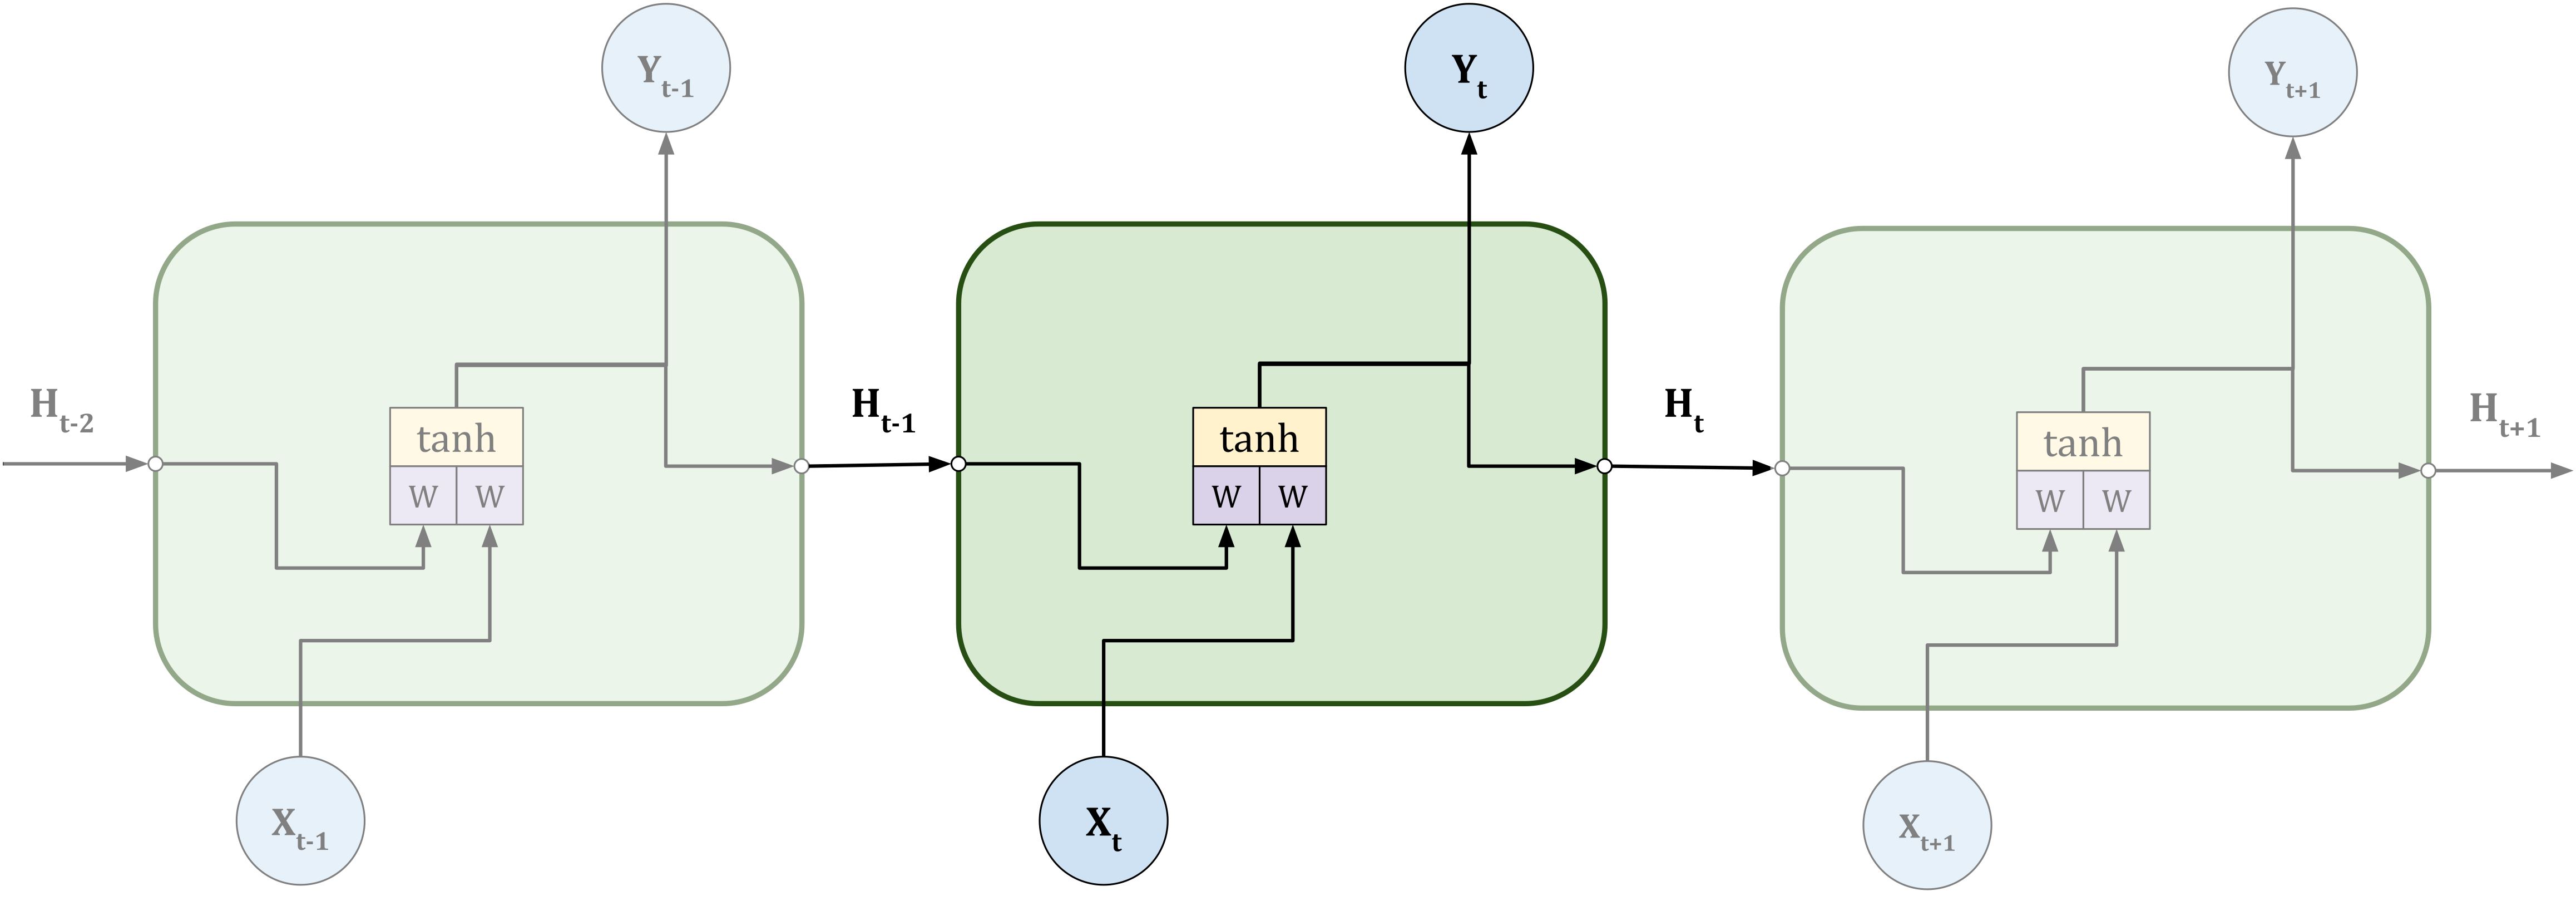
\includegraphics[width=120mm]{img/rnn_unfolded.png}
	\end{figure}

	Можно выделить три варианта конфигурации такой сети.
	
	\textbf{Sequence to sequence}
	
	Эта конфигурация применяется, когда мы хотим при помощи сети преобразовать последовательность в последовательность. Обычно это генеративная модель, например, для текстов, на каждом шаге в этом случае сеть выдаёт новую букву (вернее вектор вероятностей для букв алфавита).
	
	\begin{figure}[ht!]
		\centering
		\captionsetup{justification=centering}
		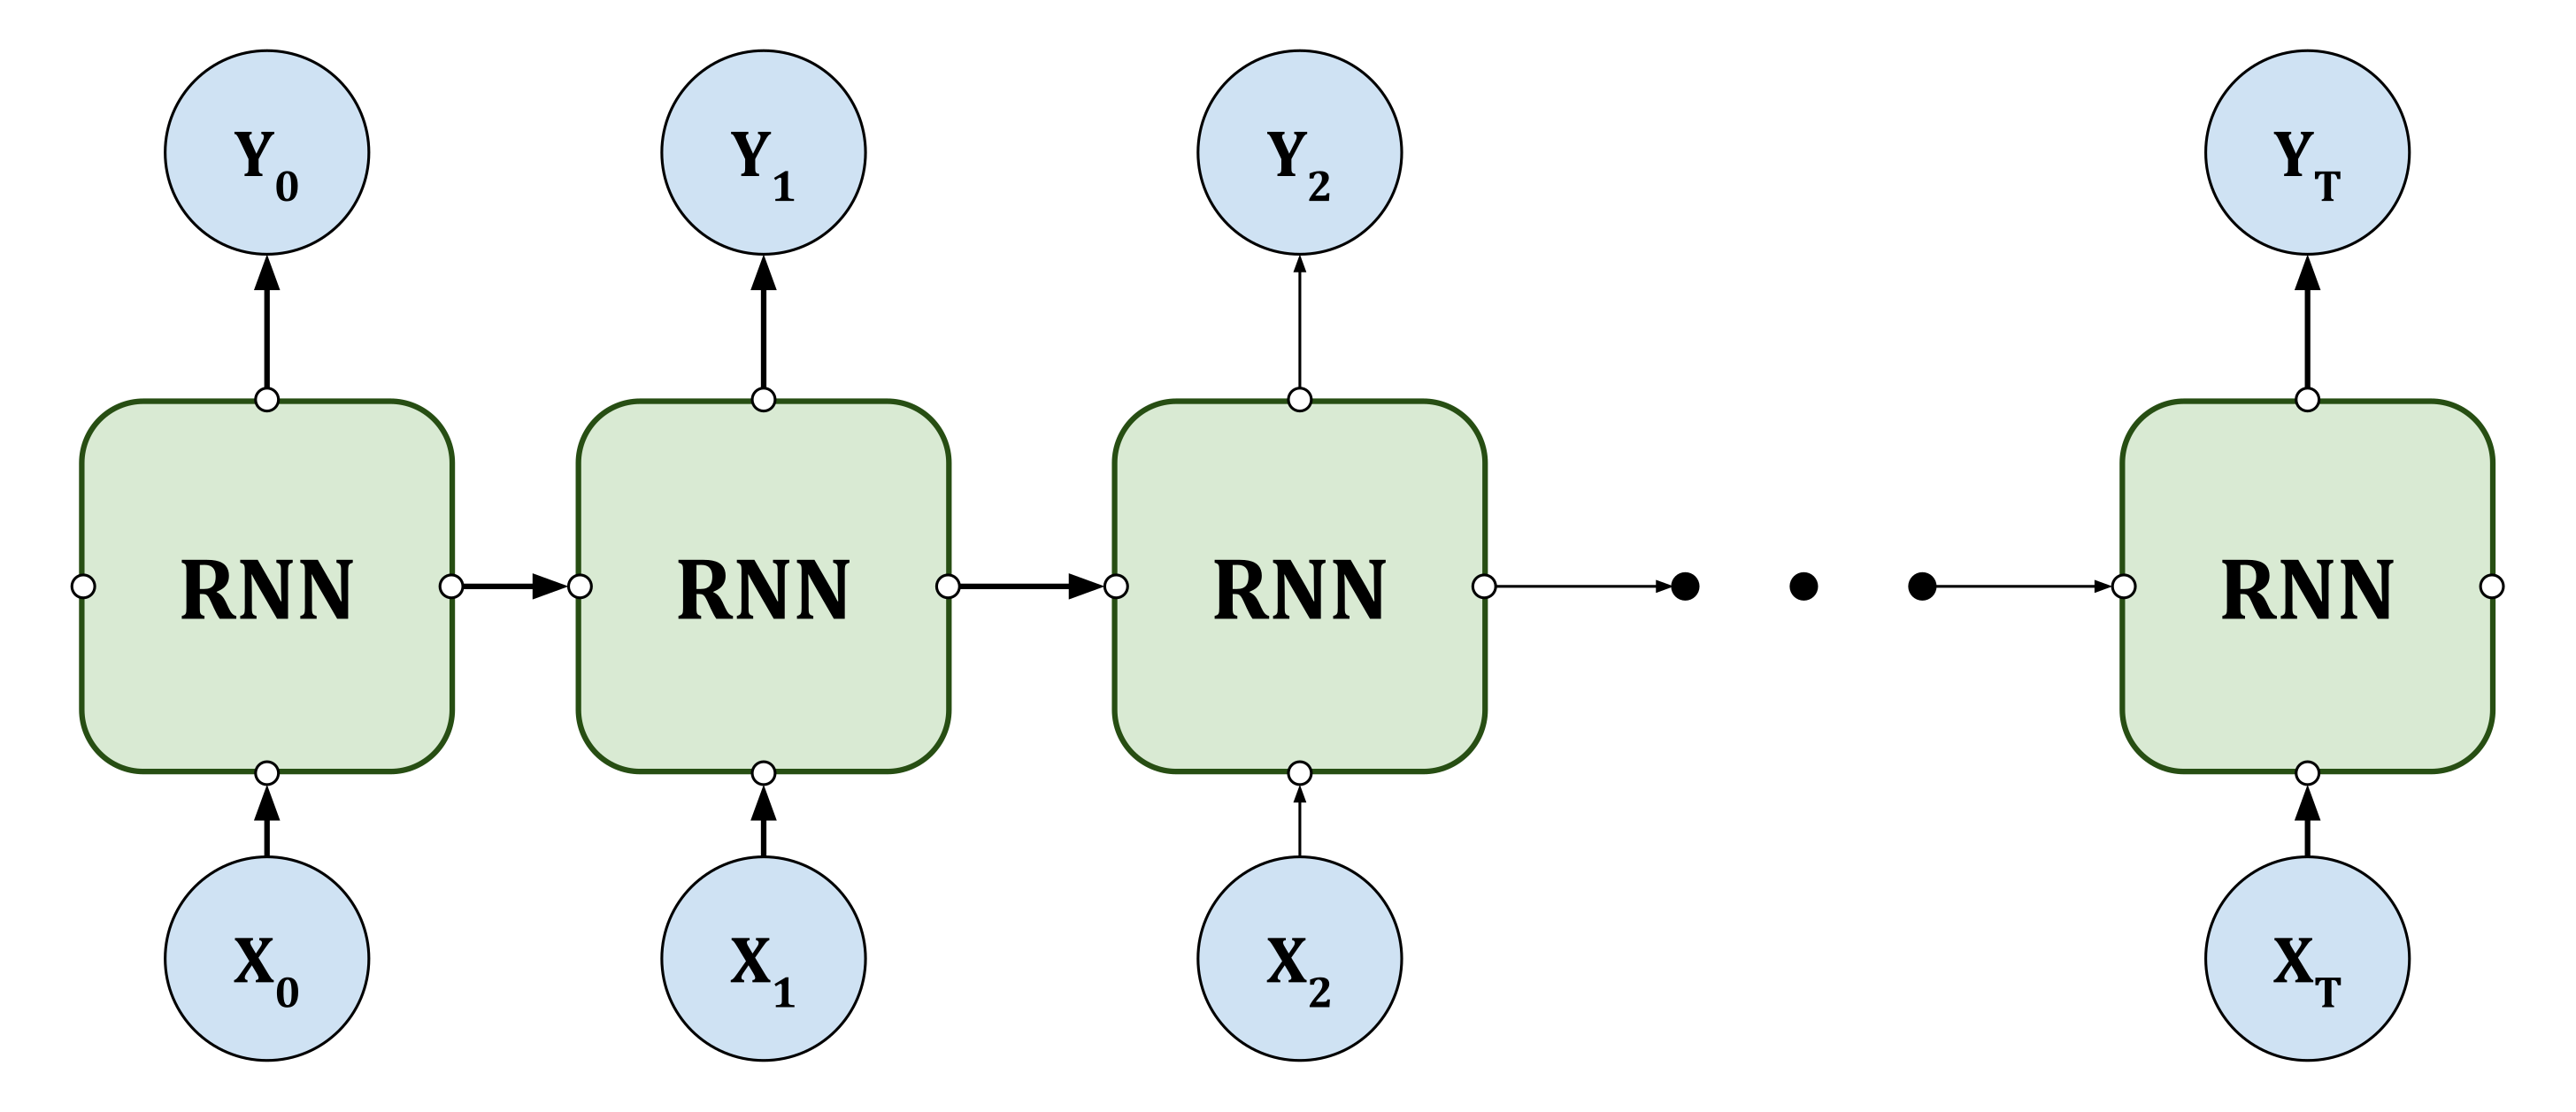
\includegraphics[height=40mm]{img/rnn_seq_to_seq.png}
	\end{figure}

	Ещё один вариант, когда сеть преобразует последовательность в последовательность, может быть вот таким:
	
	\begin{figure}[ht!]
		\centering
		\captionsetup{justification=centering}
		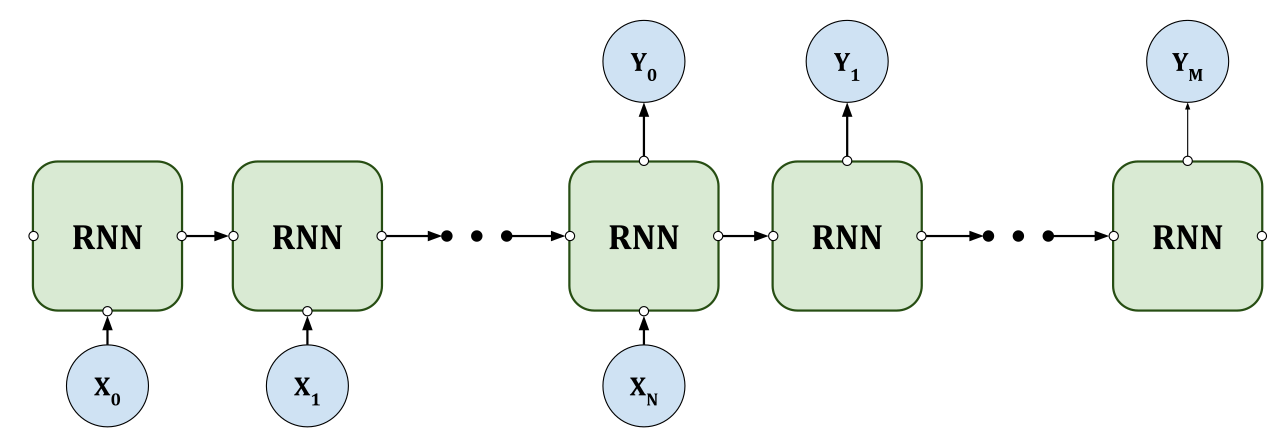
\includegraphics[height=40mm]{img/rnn_seq_to_seq_v2.png}
	\end{figure}
	
	На самом деле это сильно похоже на вариант encoder-decoder, когда входная последовательность кодируется (закодированые данные оказываются во внутреннем состоянии сети), а затем декодируется. Например, такая схема используется для переводов текстов.
	
	\textbf{Sequence to one}
	
	Эта конфигурация применима для решения задач классификации, например, текстов или видео, когда последовательность слов (или изображений) подаются на вход сети, а в качестве выхода получаем один вектор вероятностей для классов.
	
	\begin{figure}[ht!]
		\centering
		\captionsetup{justification=centering}
		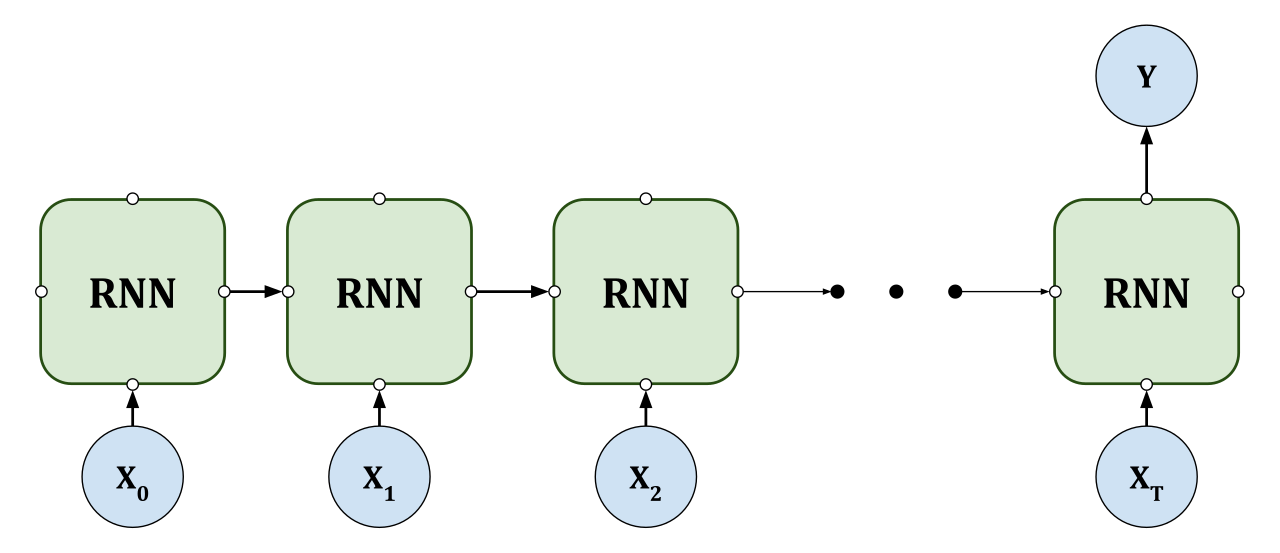
\includegraphics[height=40mm]{img/rnn_seq_to_one.png}
	\end{figure}

	\textbf{One to sequence}
	
	Ситуация обратная предыдущей, на вход приходит один элемент, а на выходе получаем целую последовательность. Например, таким образом можно генерировать текстовые подписи к изображению подаваемому на вход.
	
	\begin{figure}[ht!]
		\centering
		\captionsetup{justification=centering}
		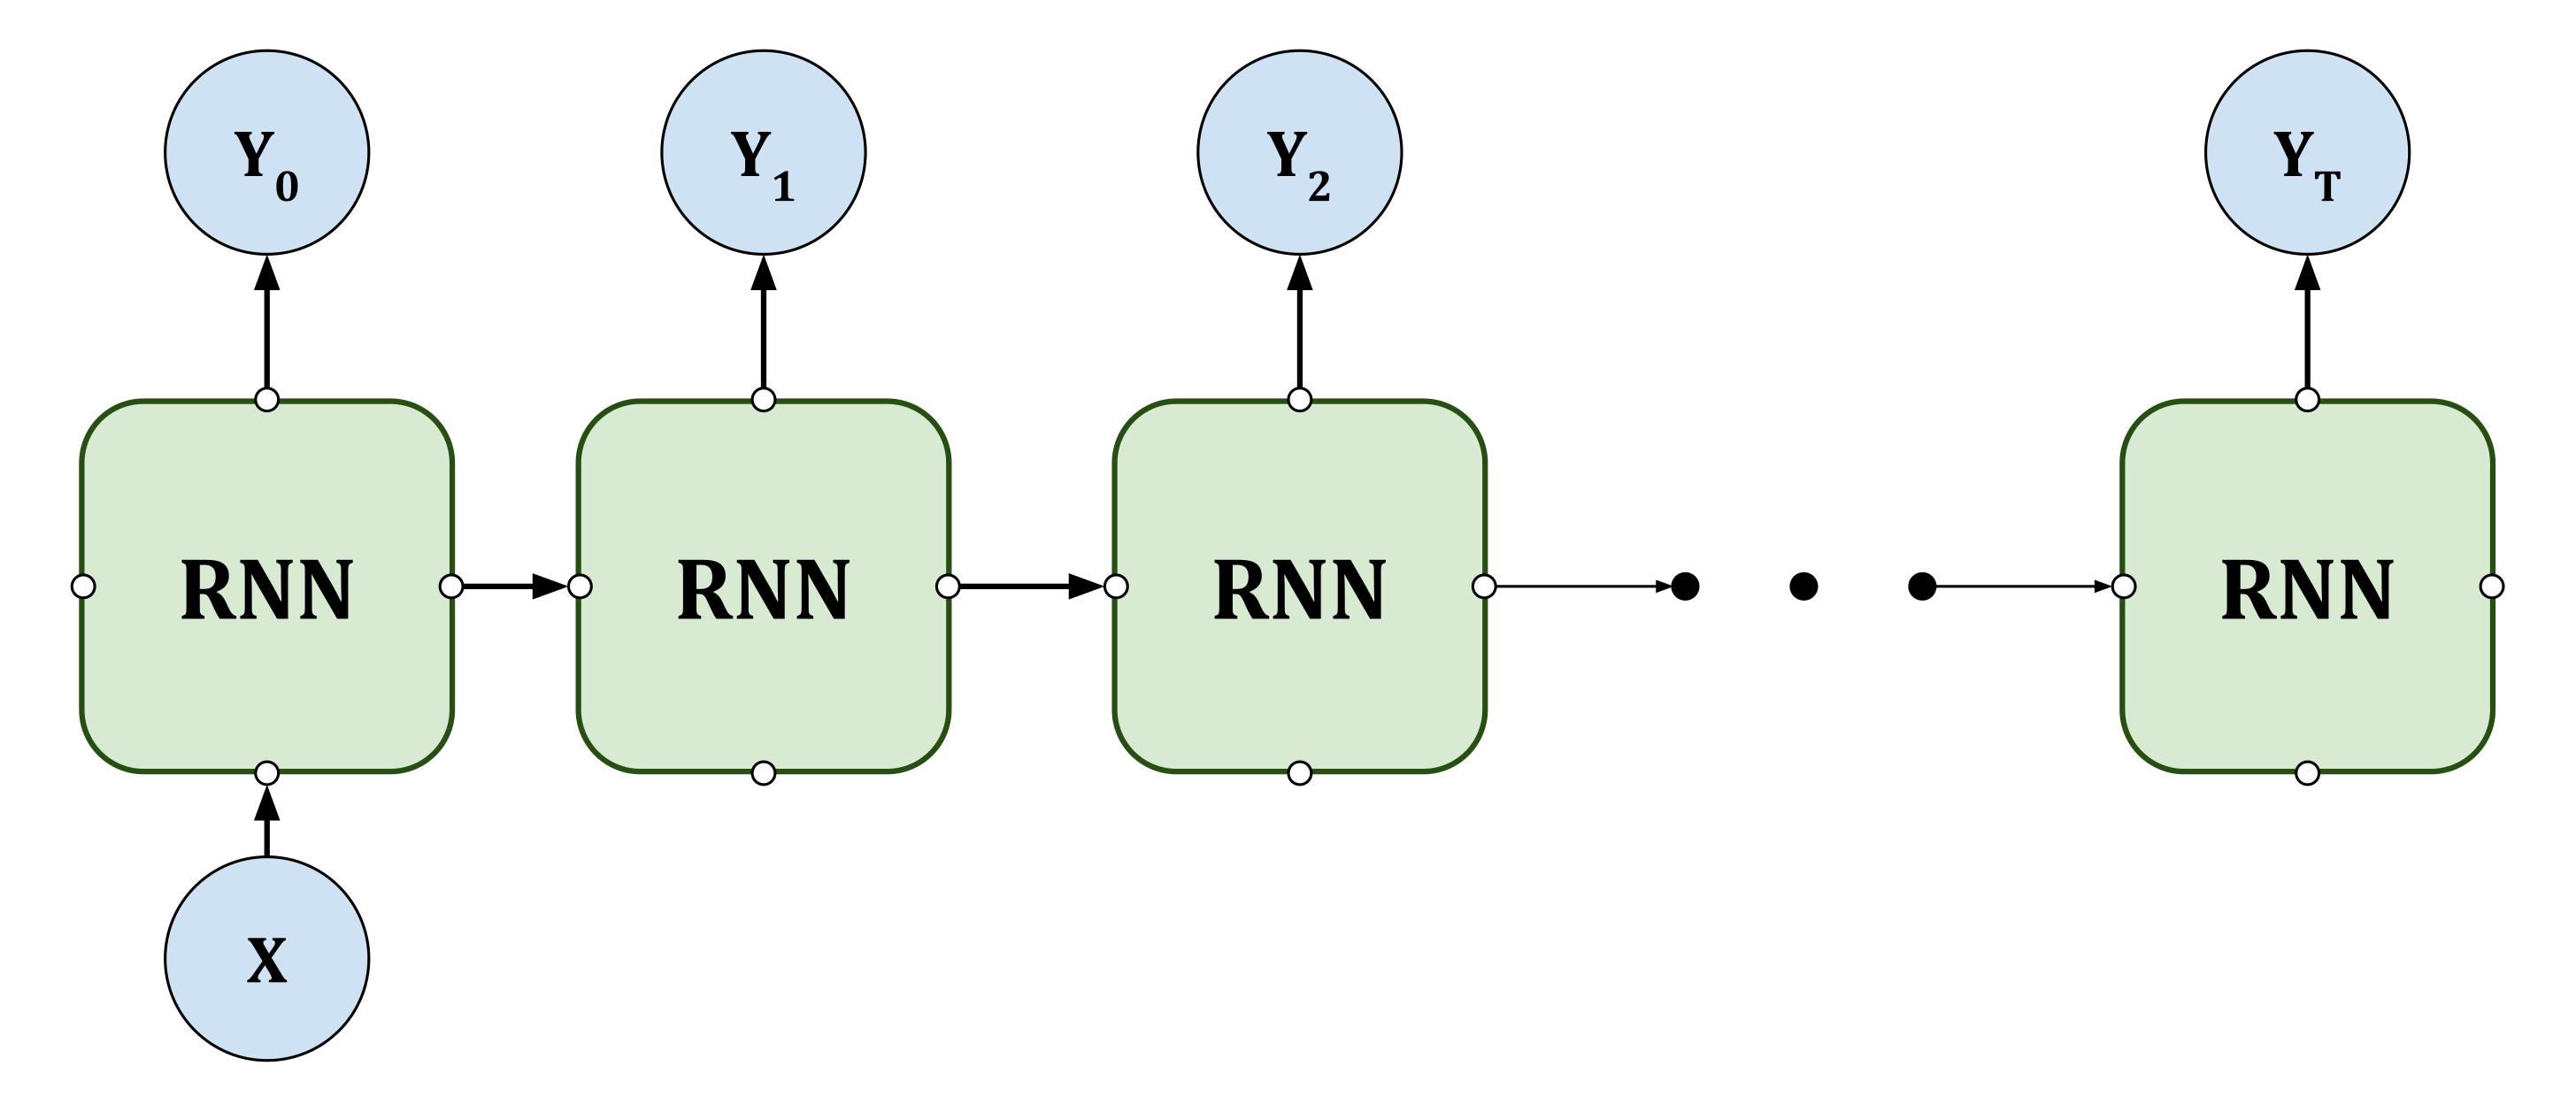
\includegraphics[height=40mm]{img/rnn_one_to_seq.png}
	\end{figure}
	
	\clearpage
	
	\subsection{LSTM - Long Short-Term Memory}
		
	\clearpage
	
	\subsection{GRU - Gated Recurrent Unit}
	
	\clearpage
	
	\section{Формализация задачи машинного перевода}
	Формально в задаче машинного перевода у нас есть входная последовательность $x_{1}, x_{2}, ... x_{m}$ и последовательность вывода $y_{1}, y_{2}, ... y_{n}$, само собой длинна данных последовательностей может отличатся. Саму процедуру \textit{перевода} можно рассматривать как нахождение искомой последовательности, которая является наиболее вероятной с учетом входных данных. Формально искомая последовательность, которая максимизирует условную вероятность $p(y|x): y^{'} = argmax[p(y|x)]$.
	
	Когда человеку известны уже два языка с которыми он работает, то уже при переводе можно сказать насколько хорошо справилась модель, является ли перевод естественным и насколько он приятен на слух. Однако такой вид анализа неприемлем для машины, поэтому нам стоит проанализировать уже имеющуюся функцию $p(y|x,\theta)$ с неким параметром $\theta$, а затем найти его $argmax$ для $y^{'} = argmax_{y}[p(y|x, \theta)]$.
	
	Прежде чем перейти к самой задачи перевода, нужно ответить на 3 вопроса:
	
	\begin{itemize}
		\item \textbf{Моделирование}: Как работает модель для $p(y|x, \theta)$?
		\item \textbf{Обучение}: Как найти параметр $\theta$?
		\item \textbf{Вывод}: Как понять, что текущий $y$ лучший?
	\end{itemize}
	
	\clearpage
	
	\section{Структура Encoder-Decoder}
	
	Наиболее распространенная модель \textbf{Sequence-to-sequence (seq2seq}) являются модель \textbf{Encoder-Decoder}, в которой обычно используют \textbf{рекуррентную нейронную сеть} (\textbf{RNN}) для кодирования исходной последовательности в один вектор.
	
	На самом деле полученный вектор можно представить как набор образов сущностей с образами взаимоотношений между ними. Этот вектор затем декодируется вторым \textbf{RNN}, который учится выводить выходное предложение, генерируя его по одному слову за раз.
	
\end{document}